% ****** Start of file aipsamp.tex ******
%
%   This file is part of the AIP files in the AIP distribution for REVTeX 4.
%   Version 4.1 of REVTeX, October 2009
%
%   Copyright (c) 2009 American Institute of Physics.
%
%   See the AIP README file for restrictions and more information.
%
% TeX'ing this file requires that you have AMS-LaTeX 2.0 installed
% as well as the rest of the prerequisites for REVTeX 4.1
% 
% It also requires running BibTeX. The commands are as follows:
%
%  1)  latex  aipsamp
%  2)  bibtex aipsamp
%  3)  latex  aipsamp
%  4)  latex  aipsamp
%
% Use this file as a source of example code for your aip document.
% Use the file aiptemplate.tex as a template for your document.
\documentclass[%
 aip,
% jmp,
% bmf,
% sd,
% rsi,
 amsmath,amssymb,
%preprint,%
 reprint,%
%author-year,%
%author-numerical,%
% Conference Proceedings
]{revtex4-1}

\usepackage{graphicx}% Include figure files
%\usepackage{dcolumn}% Align table columns on decimal point
\usepackage{bm}% bold math
\usepackage{fixme}
%\usepackage[mathlines]{lineno}% Enable numbering of text and display math
%\linenumbers\relax % Commence numbering lines
\usepackage{hyperref}
\usepackage{kbordermatrix}% http://www.hss.caltech.edu/~kcb/TeX/kbordermatrix.sty
\usepackage[utf8]{inputenc}
\usepackage[T1]{fontenc}
\usepackage{mathptmx}
\usepackage{lipsum}
\usepackage{amsmath}
\usepackage{physics}
\usepackage{xparse}
\usepackage{bbm}
\usepackage{xcolor}


%\usepackage{multirow}
%\usepackage{makecell}
\graphicspath{{Pictures/}}

\renewcommand*{\figureautorefname}{Fig.}

\newcommand{\mytitile}{Effects of strong interaction between light and matter in a superconducting artificial molecule}

\begin{document}
	\preprint{AIP/123-QED}
	
	\title[\mytitile]{\mytitile\\~}
	
	\author{G.P. Fedorov}
	\email{gleb.fedorov@phystech.edu}
	
	\affiliation{ 
		Russian Quantum Center, Skolkovo village, Russia
	}%
	\affiliation{ 
		Moscow Institute of Physics and Technology, Dolgoprundiy, Russia
	}%
	
	\author{V.B. Yursa}
	\affiliation{ 
		Moscow Institute of Physics and Technology, Dolgoprundiy, Russia
	}%
	
	\author{A. Efimov}
	
	\affiliation{ 
		Moscow Institute of Physics and Technology, Dolgoprundiy, Russia
	}%
	
	\author{K. Shiianov}

	\affiliation{ 
		Moscow Institute of Physics and Technology, Dolgoprundiy, Russia
	}%

	\author{A. Yu. Dmitriev}
	\affiliation{ 
	Moscow Institute of Physics and Technology, Dolgoprundiy, Russia
	}%

	\author{O.V. Astafiev}
	\affiliation{ 
		Moscow Institute of Physics and Technology, Dolgoprundiy, Russia 
	}%
	
	
	\date{\today}% It is always \today, today,
	%  but any date may be explicitly specified
	
	
	\begin{abstract}
		To build a full-scale quantum processor it is necessary to automate as many steps as possible on the physical, hardware level. Circuit quantum electrodynamics (cQED) is a contemporary architecture for dispersive readout and Purcell protection of superconducting qubits of various types, and thus it is necessary to develop software that is able to perform every kind of automatic calibration of such systems from scratch without any human participation. An important step towards this goal is to build a noise-insensitive and accurate computer vision tool to process three-dimensional spectroscopic data. In this work, we present and describe two scalable algorithms that are able to extract the Hamiltonian parameters of the cQED systems from spectroscopic data. 
	\end{abstract}
	
	\maketitle
\section{Introduction}


Over the past twenty years, superconducting artificial atoms (SAA) were used in numerous experiments confidently demonstrating the validity of fundamental quantum mechanical laws\cite{you2011atomic}. Due to synthetic nature of SAA, their Hamiltonians can be pre-designed and engineered, and this makes them a particularly versatile tool for studies in quantum optics. Notably, their parameters may be varied in such a wide range that novel physical effects previously inaccessible for natural systems may be directly observed. For example, the strong coupling regime when the coupling strength between light and a quantum system approaches 1\% of their frequency has been a major milestone for atoms, molecules, etc and was only reached using high-finesse cavities. In contrast, superconducting quantum systems have rapidly attained this landmark using \textit{circuit QED}\cite{wallraff2004strong} just in a few years after their first discovery\cite{chiorescu2004coherent} and have already surpassed other strongly-coupled systems in terms of coherence\cite{forn2019ultrastrong}. 
Moreover, SAA do not even require confined radiation to implement strong coupling with light: they may be coupled unprecedently strong with the free-propagating EM-waves in the on-chip 1D waveguides\cite{astafiev2010resonance} without having to use cavities at all. The Rabi frequency in this case may reach 50\% of the transition frequency\cite{deng2015observation} which is already the ultra-strong coupling regime.

In general, a quantum system exposed to strong external driving can experience various quantum phenomena explained by resonant single- and multi-photon transitions between energy levels. The most known examples are coherent population trapping, electromagnetically induced transparency (EIT)\cite{boller1991observation}, stimulated Raman adiabatic passage\cite{bergmann1998coherent} and Autler-Townes (A-T) splitting\cite{autler1955stark}. 

In this work, we are studying effects of light-matter interaction that occur in a system of two coupled artificial atoms: a superconducting artificial molecule (SAM). In our experiment, we use two transmons\cite{koch2007charge} interacting with each other through a cavity bus\cite{majer2007coupling}. Microwave radiation is applied to this system through a coplanar on-chip antenna and transmon states may be monitored by dispersive readout using the same coupling cavity \cite{chow2010detecting}.


It turns out that due to the strong interaction of SAM with the microwave drive, multiphoton transitions and the Autler-Townes effect are playing the crucial role in the phenomena that we have discovered. The A-T splitting has been observed before in atomic\cite{picque1976direct}, molecular systems\cite{tamarat1995pump}, quantum dots\cite{xu2007coherent}, and for SAA as well\cite{baur2009measurement, sillanpaa2009autler, novikov2013autler, suri2013observation, peng2018vacuum}. However, the previous studies have  only involved just a single SAA and have demonstrated only the standard spectral signatures known from the quantum optics (see Appendix \ref{sec:3-level-at}); instead, a diatomic SAM allows to observe some qualitatively new spectral manifestations of the effect. Remarkably, besides its fundamental value, this experiment may be useful for future quantum computers: a quantum engineer should consider the observed behaviours as unwanted, and thus careful control of the driving power must be employed to avoid them (for instance, as we will show, the bSWAP gate\cite{poletto2012entanglement} is directly affected).

The manuscript consists of four main parts and an Appendix. Section I is this introduction; Section II is devoted to the approaches that were used in our study; Section III contains the results of our experimental and theoretical research; finally, in Section IV we make a conclusion of our work and discuss future prospects. The Appendix contains important details of the theoretical framework that we use.

\section{Methods}

\subsection{Device design and fabrication}
We have designed the SAM as a pair of transmon (Xmon\cite{barends2013coherent}) SAAs with asymmetric SQUIDs\cite{hutchings2017tunable} coupled to a single notch-type\cite{probst2015efficient} $\lambda/4$ resonator ($\omega_r/2\pi \equiv f_r = 7$ GHz, $\kappa = 1/100\ \text{ns}^{-1}$) which both couples\cite{majer2007coupling} the qubits and allows the joint\cite{chow2010detecting} readout of their states. In \autoref{fig:experiment}~(a), the optical photograph of the device is shown depicting the layout of the components. The resonator in its upper part is connected to a coplanar waveguide through which the readout is performed. In its lower part, it is coupled to the transmons by a dual ``claw''\cite{barends2013coherent} coupler. Flux lines that allow independent control of the transmon frequencies are coming from the sides. Finally, the excitation waveguide coming from below directs microwave signal towards the SAM. In \autoref{fig:experiment}~(b) the equivalent electrical circuit of the device. The resonator fundamental mode is approximated as an LC-circuit (in the middle), the transmons are shown in colour on the sides as the LC-circuits as well, but with tunable non-linear inductances. The capacitively coupled excitation line is also shown in green. Finally, in \autoref{fig:experiment}~(c) we show schematically the frequencies of the transmons depending on the external magnetic flux. Since the effective junction of the first transmon is larger, its spectrum (orange) lies higher in frequency the spectrum of the second qubit (blue). Using both coils, it is possible to align them so that the lower sweet-spot of the orange transmon is just below the upper sweet-spot of the blue transmon (see the dashed rectangle,  \autoref{fig:experiment}~(c)). This configuration is chosen as it is possible to track higher energy level intersections through multi-photon transitions using a single spectroscopic scan since the transmons are staying close to each other in frequency. Additionally, the transmons are better protected from the flux noise in this area being close to their sweet spots.

The fabrication process...


\begin{figure}
	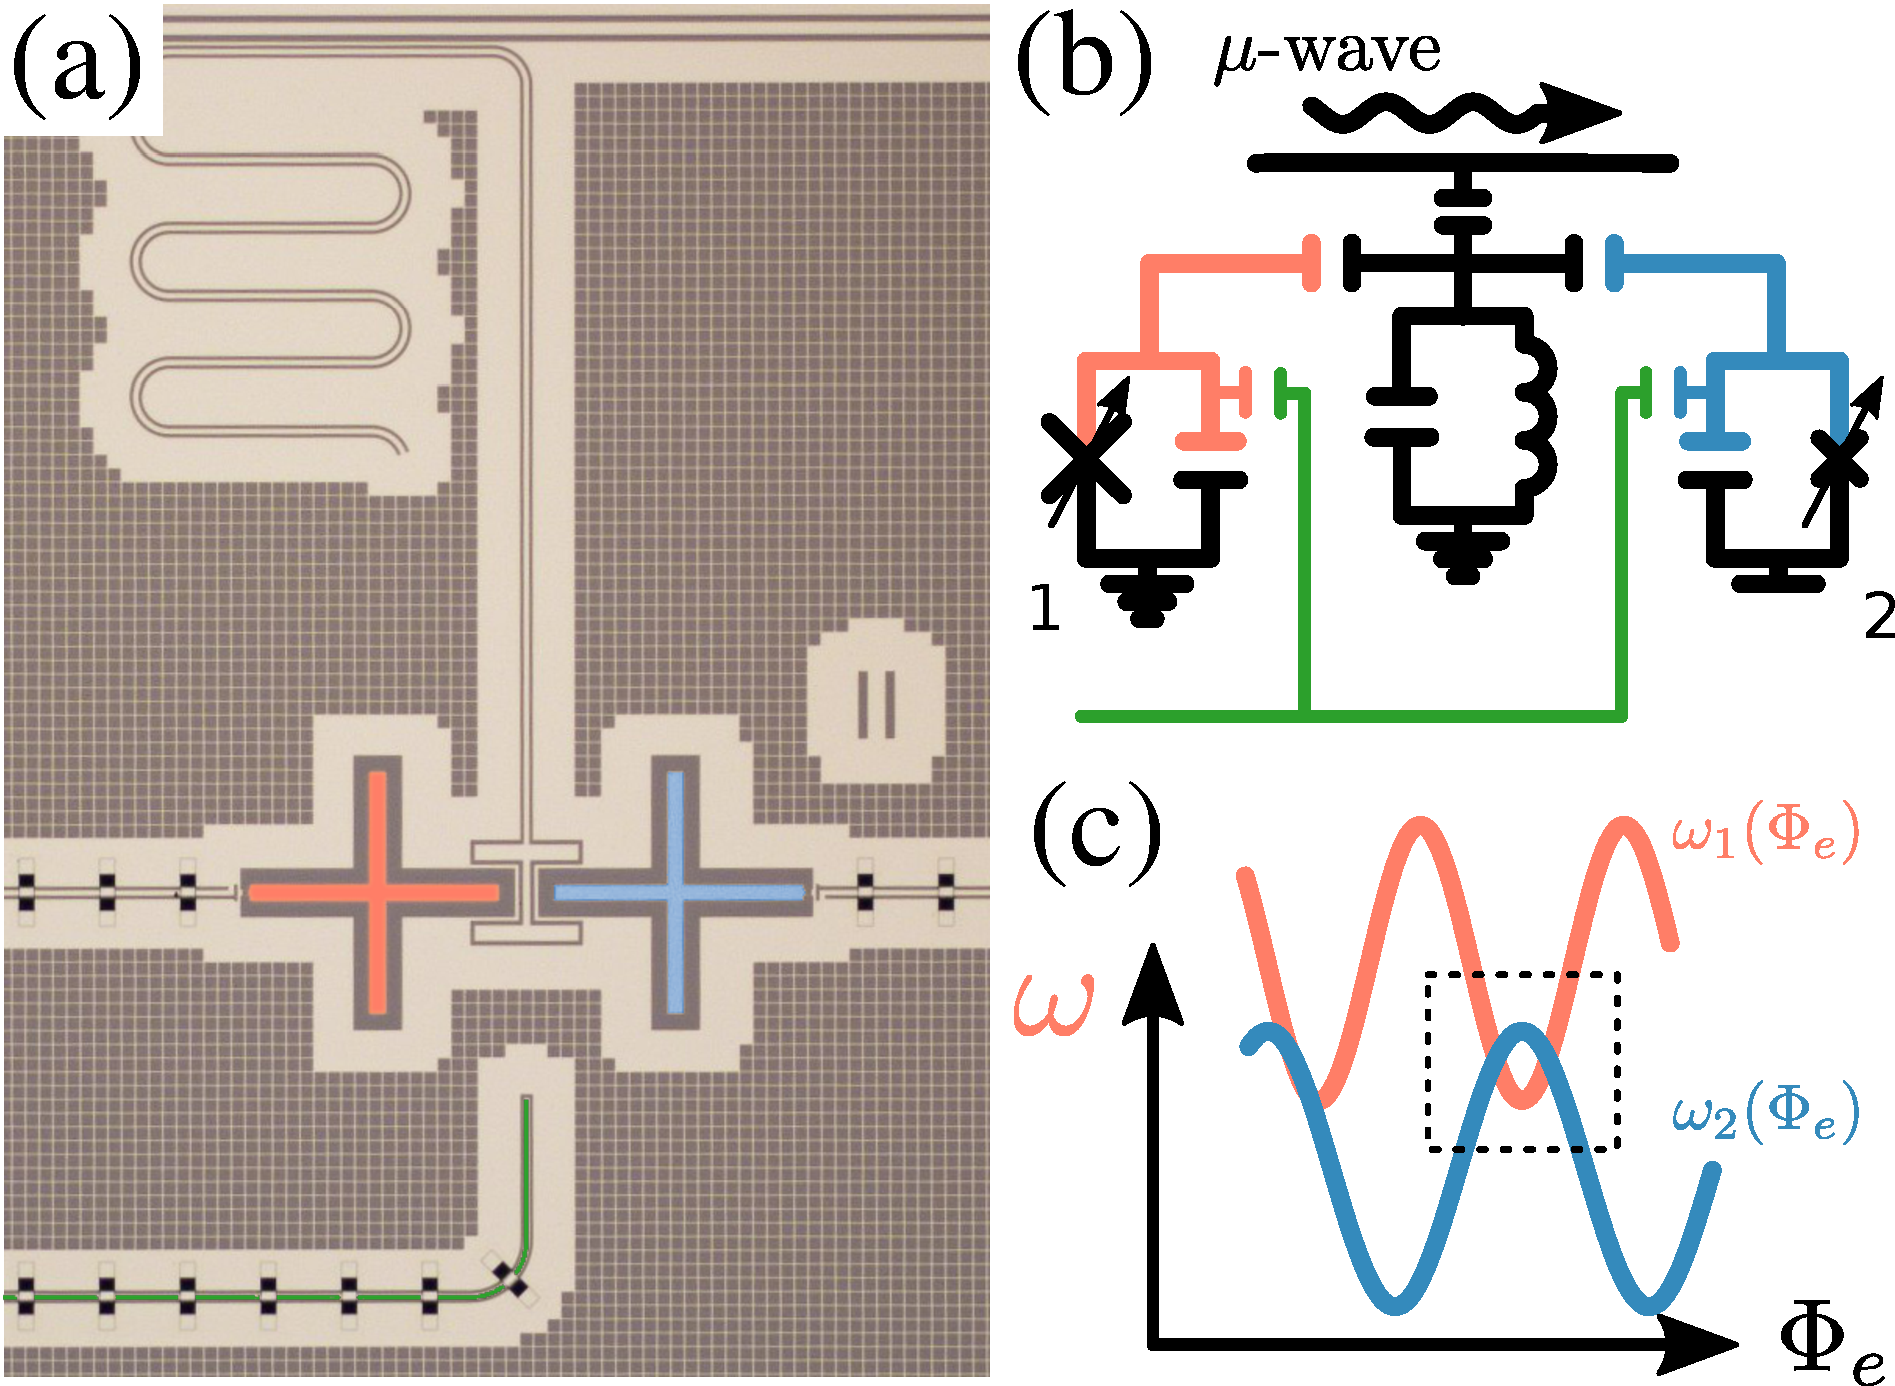
\includegraphics[width=\linewidth]{experiment_2}
	\caption{\textbf{(a)} Optical photograph of the device (false coloured). Two transmons (orange, 1 and blue, 2) are coupled capacitively to a $\lambda/4$ coplanar resonator. From both sides come the frequency control flux lines, and from below a microwave excitation waveguide is connected (green). \textbf{(b)} The equivalent electrical circuit. Tunable Josephson junctions are in fact SQUIDs with magnetic flux control. \textbf{(c)} Frequencies of the $ge$ transitions of the transmons $\omega_1(\Phi_e)$ and $\omega_2(\Phi_e)$ depending on the external magnetic flux (coloured correspondingly). In this work, we concentrate on the area inside the dashed rectangle.}
	\label{fig:experiment}
\end{figure}


\begin{table}
	\begin{ruledtabular}
	\begin{tabular}{rll}
	Parameter & Transmon 1  & Transmon 2\\\hline
	$\omega/2\pi$ [GHz] & 5.12 - 6.3  & 4 - 5.45\\
	$\alpha/2\pi$ [MHz] & 220 & 220 \\
	$T_1$ [$\mu$s]  & 6.82 &  4.41 \\
	$T_2^*$ [$\mu$s]  & 5.14  &  3.33\\\hline
	$J/2\pi$ [MHz] &\multicolumn{2}{c}{10} 
	\end{tabular}
	\end{ruledtabular}
	\caption{SAM parameters. Transmons are only different in the frequency tuning range and coherence times measured in the lower sweet spot for the 1\textsuperscript{st} one and in the higher sweet spot for the 2\textsuperscript{nd}.}
\end{table}


\subsection{Theoretical description of the SAM}

A single transmon SAA can be considered as an oscillator with a quartic perturbation describing the leading-order anharmonicity. Therefore, in the main text we avoid using the standard charge and phase operators and write down its Hamiltonian using the annihilation operator $\hat b$ ($\hbar = 1$):
\begin{equation}
\hat{{H}}_{tr} = \omega \hat b^{\dagger}\hat b +\frac{1}{2}\alpha \hat b^{\dagger}\hat b(\hat b^{\dagger}\hat b-1),
\end{equation}
where $\omega$ is its $\ket{0}\rightarrow\ket{1}$ (or the  $ge$) transition frequency and $\alpha$ is the anharmonicity of the transmon. Additionally, by applying external magnetic flux $\Phi_e$ (via a control current) it is possible to control $\omega = \omega(\Phi_e)$\cite{koch2007charge}. In our modelling, we take into account only the three lowest states of the transmon ($\ket{0},\ \ket{1}$ and $\ket{2}$).

To induce state transitions in a transmon one should irradiate it by a monochromatic microwave signal of frequency $\omega_d$ using a capacitively coupled transmission line. The interaction term between the transmon and the field is then modelled by the following operator: 
\begin{equation}
\hat H_{d} = \Omega (\hat b+\hat b^{\dagger}) \cos\omega_d t,
\end{equation}
where $\Omega$ stands for the frequency of the Rabi oscillations between $\ket{0}$ and $\ket{1}$.

Now, the complete Hamiltonian of SAM contains two terms describing each of them in isolation (with the corresponding annihilation operators $\hat b$ and $\hat c$, the $ge$ frequencies $\omega_{1,2}$ and anharmonicities $\alpha_{1,2}$), two terms representing the interaction of each transmon with the driving field at the same frequency $\omega_d$, and the transmon-transmon interaction term:
\begin{equation}\label{Hsystem}
\hat H = \hat H_{tr1}+\hat H_{tr2}+\hat H_{d}^1+\hat H_{d}^2+\hat H_{int},
\end{equation}
where $\hat H_{int} = J (\hat b +\hat b^\dag)(\hat c+\hat c^{\dagger})$ is the transverse interaction between the atoms. In the following, we will also transform \eqref{eq:master} into the frame rotating with both drives by an operator
\begin{align}
&\hat R = \exp[-i t (\omega_d^1 b^{\dagger}b+\omega_d^2 c^{\dagger}c)],\label{eq:R}\\
&\hat H_R = \hat R^{\dagger}\hat H \hat R - i\hat R^{\dagger}\partial_t \hat R.\label{eq:rotation}
\end{align}
After the transformation and application of the RWA:
\begin{equation}
\begin{aligned}
	\omega_{(1,2)} &\rightarrow \Delta_{(1,2)} = \omega_{(1,2)} - \omega_d^{(1,2)},\\
	\hat H_{int} &\rightarrow J \left[\hat b^\dag \hat c e^{-(\omega_d^1 - \omega_d^2)t} + \hat b \hat c^\dag e^{(\omega_d^1 - \omega_d^2)t}\right],\\
	\hat H_{d}^1 &\rightarrow \frac{\Omega_1}{2}(\hat b  + \hat b^\dag),\ 	\hat H_{d}^2 \rightarrow \frac{\Omega_2}{2}(\hat c  + \hat c^\dag).
\end{aligned}
\label{eq:RWA}
\end{equation}

Besides the unitary evolution, we take into account the incoherent processes of relaxation and dephasing for each transmon. They are modelled using the Lindblad equation with the following collapse operators:
\begin{equation}\
\begin{split}
\hat{{O}}_{\gamma, 1} = \sqrt{\gamma_1}\, \hat b,\ 
\hat{{O}}_{\phi, 1} = \sqrt{2\gamma_{\phi,1}}\, \hat b^\dag \hat b,\\
\hat{{O}}_{\gamma,2} = \sqrt{\gamma_2}\, \hat c,\ 
\hat{{O}}_{\phi,2} = \sqrt{2\gamma_{ \phi,2}}\, \hat c^\dag \hat c.
\end{split}
\end{equation}
As one can see, the collapse operators are in a separable form, i.e. acting only upon a single transmon each. This is a valid approach until the coupling strength $J$ is not too large\cite{beaudoin2011dissipation}. Therefore, the complete evolution equation for the system density matrix $\hat \rho$ is
\begin{equation}
\partial_t \hat \rho = {i}[\hat \rho, \hat H] + \sum_{\alpha, i} \mathcal{D}[\hat{O}_{\alpha, i}] \hat \rho = \mathcal{L}\hat\rho, \label{eq:master}
\end{equation}
where $\mathcal{D}[\hat{{O}}]\hat \rho = \hat{{O}} \hat \rho \hat{{O}}^\dag - \frac{1}{2}\{ \hat{{O}}^\dag \hat{{O}}, \hat \rho\}$ and $\mathcal{L}$ is the Liouville superoperator or the Liouvillian.


The readout resonator is not included in the model since in the dispersive regime is does not affect the dynamics of the SAM. Hence, the readout is modelled just by using the measurement operator $\hat M(f_p)$ that can be obtained by measuring the transmission $S_{21}(f_p)$ ($f_p$ is the probe frequency near the resonance) through the sample for the nine different states of the SAM $\ket{ij},\ i=0..2,\ j=0..2$\cite{filipp2009two}. Another way to find $\hat M(f_p)$ is to calculate the transmission by offsetting the experimental resonance curve using the dispersive shifts corresponding to these states. Since we have not directly measured the dispersive shifts, in our modelling they are treated as fitting parameters. Finally, the observable value for any state $\hat \rho$ is calculated as $S_{21}^{sim}(f_p) = \Tr[\hat M(f_p) \hat \rho]$.


\subsection{Numerical solution in \textit{qutip}}


Numerical simulations are crucial for studying the equation \eqref{eq:master} since is does not allow  analytical solution. Therefore, we have been using the \textit{qutip}\cite{johansson2013qutip} (quantum optics toolbox) to simulate the dynamics and find the steady state of the system for various parameter combinations of the Liouvillian.

Two distinct modes of simulation were used during the modelling. The first one is for the Liouvillians that do not explicitly depend on time (stationary case). In this case, the steady state $\hat \rho_{ss}$ of the system should be calculated from the set of linear equations obtained from \eqref{eq:master}:
\begin{equation}
\partial_t \hat \rho = 0 = \mathcal{L} \hat \rho
\end{equation}
This equation is solved with the qutip's \textit{steadystate} function\footnote{http://qutip.org/docs/4.0.2/guide/guide-steady.html}. This method is applicable when the driving of the two transmons is at the same frequency since from \eqref{eq:RWA} follows that $\hat H_{int}$ becomes time independent when $\omega_d^1 = \omega_d^2$.

The second mode is required when it is not possible to avoid the time-dependence of the Liouvillian. This is the case when the transmons have to be excited at different frequencies ($\omega_d^1 - \omega_d^2 = \delta \neq 0$). From \eqref{eq:RWA} we find that even in the doubly-rotating frame $\hat H_{int}$ is oscillating, and it is not possible to simply drop this term in RWA because this will lead to qualitatively different results. In this case, to find the steady state of the system we employ the qutip's \textit{propagator} and \textit{propagator\_steadystate} functions. The propagator is a completely positive map $\Lambda(t_1, t_0): \hat \rho(t_0) \rightarrow \hat \rho(t_1)$ describing the time evolution of the system density matrix; for \eqref{eq:master}, it is defined as
\begin{equation}
\Lambda(t_1, t_0) = \mathcal{T} \exp [\int_{t_0}^{t_1} \mathcal L(\tau) d\tau],
\label{eq:propagator}
\end{equation}
where $\mathcal T$ is the time-ordering superoperator. Since the Liouvillian is periodic with a period of $T = 2\pi/\delta$, it is possible to calculate the steady state as the eigenvector $\hat \rho_{ss}$ of the single-period propagator $\Lambda(T, 0)$ corresponding to its largest eigenvalue\cite{dittrich1998quantum, rivas2012open}. Upon infinite applications of $\Lambda$: 
\[
\lim_{n\to \infty} \left[\Lambda(T, 0)\right]^n \hat \rho = \Lambda(nT, 0) \hat \rho \to \hat \rho_{ss}.
\]


\section{Results}

\subsection{\label{sec:level1} Spectroscopy: experiment and numerical simulation}

\begin{figure*}
	
	\centering
	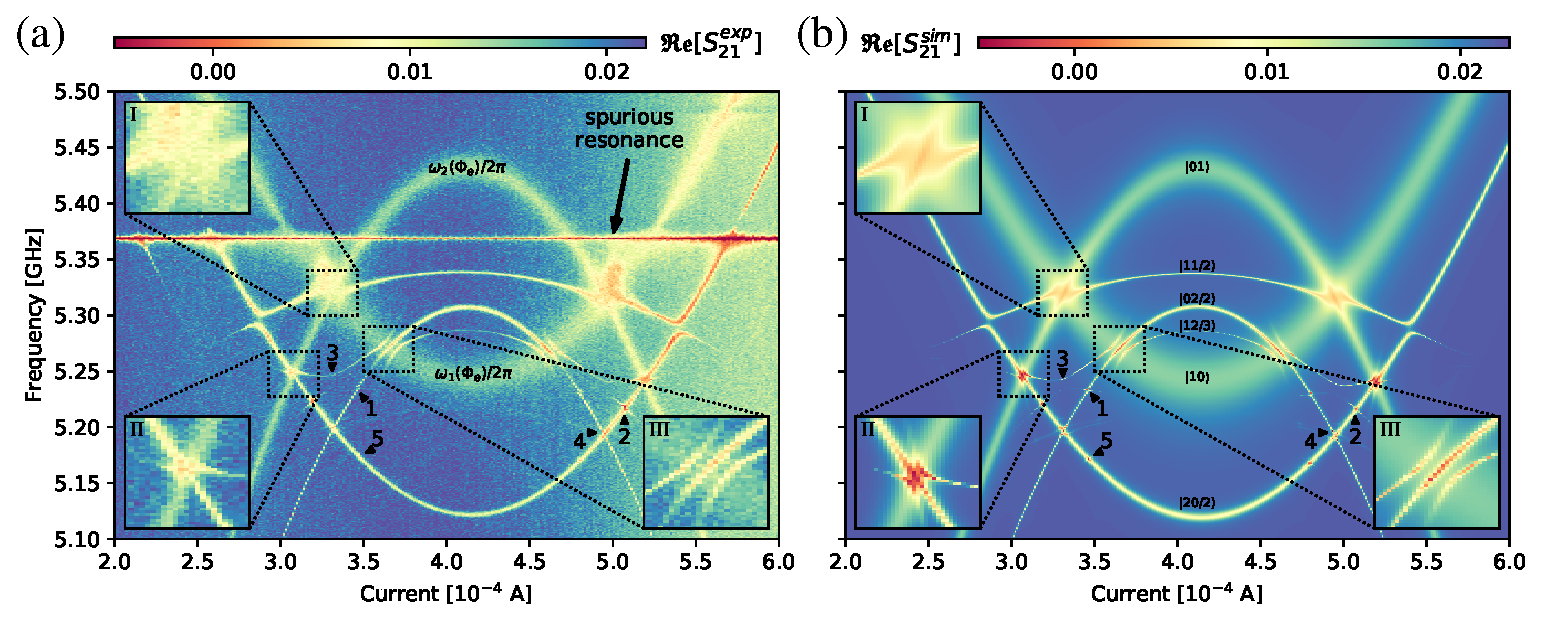
\includegraphics[width=\linewidth]{main_picture}
	\caption{Two-tone spectroscopy: experiment \textbf{(a)} and numerical modelling \textbf{(b)}. Colour shows the real part of complex transmission  through the sample. Two transmons are aligned as in \autoref{fig:experiment}~(c) and form a symmetric picture. Experimental data contain an additional horizontal line from a parasitic resonance interacting with the readout resonator. Three avoided crossings not predicted by the stationary model are shown in insets I, II and III; other pronounced features reproduced by the modelling are shown with numbered markers (see text for description). We also denote some of the transitions $00 - ij/n$ where $i,j$ stand for the final transmon energy levels and $/n$ is optional for an $n$-photon process.}
	\label{fig:two-tone}
\end{figure*}


\begin{figure}
	\centering
	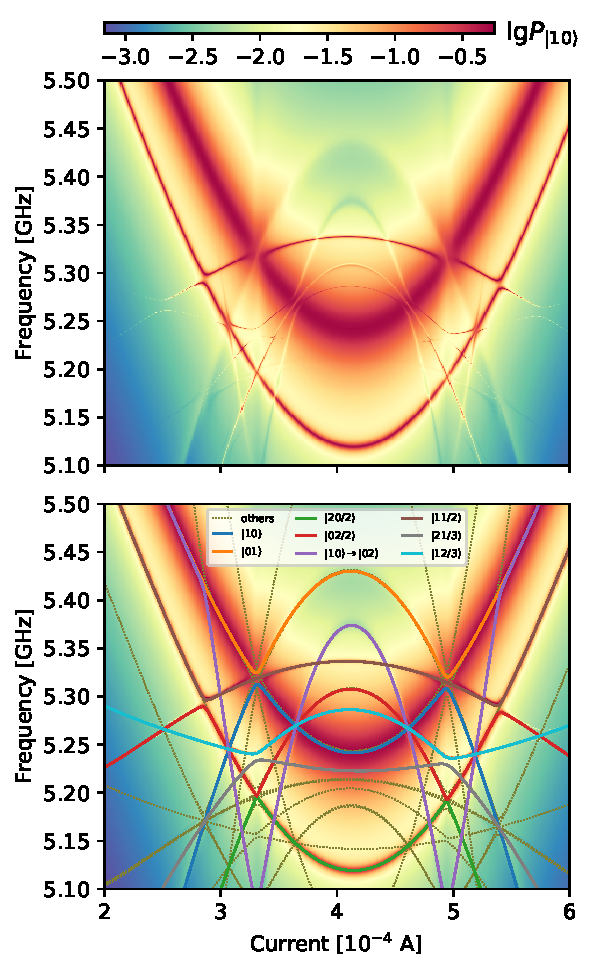
\includegraphics[width=\linewidth]{stationary}
	\caption{Simulated population of the first qubit excited state ($\lg P_{\ket{10}}$ is shown with colour). Lines show various transition frequencies from the stationary Hamiltonian. The legend labels the transitions at the sweet spot current; if elsewhere any two lines cross, the labels should be swapped after the intersection.}
	\label{fig:statinary_levels}
\end{figure}


Experiment was conducted as described in Appendix \ref{sec:meas_setup}. We have used high-power two-tone spectroscopy to probe transitions between eigenstates of our SAM; the result is shown in \autoref{fig:two-tone}~(a). As one can see, several spectral lines are visible besides the $ge$ ones shown in \autoref{fig:experiment}~(c). Their frequency depends on the applied current, and at multiple points they become resonant with each other. At three pairs of these resonant points, we observe distinct features shown in insets marked with Roman numerals. Some secondary details are shown with Arabic-numbered markers.

Remarkably, in areas I, II and III we could observe avoided crossings and triplet transitions which turn out to be impossible to explain using only the stationary Hamiltonian without driving terms. We confirm this by numerically diagonalizing $\hat H_{tr1}+\hat H_{tr2}+\hat H_{int}$ taking 3 levels for each transmon (and total 9 basis states of SAM); all possible transitions between all eigenlevels of the SAM are shown in \autoref{fig:statinary_levels}. While correctly reproducing, for instance, the avoided crossing labelled as feature 3 in \autoref{fig:two-tone}~(a), it completely misses the Roman-numbered effects. Taking into account more energy levels for transmons does not help, and is not even necessary to reproduce the experiment, as we will show in the following.

To check whether the described features are present in the dynamic regime, we have solved the master equation \eqref{eq:master} to find the steady states of the system $\hat \rho_{ss}$ and the corresponding expected measurement outcomes $\mathfrak{Re}\left[\Tr[\hat M \hat \rho_{ss}]\right]$ depending on the excitation frequency and magnetic flux. Strikingly, all the experimental features are immediately reproduced using this approach with just 9 SAM states as shown in \autoref{fig:two-tone}~(b). We have solved \eqref{eq:master} with and without RWA (using the propagator approach \eqref{eq:propagator}) and did not find any noticeable difference in the results; though, the runtime of a single 401 by 401 points simulation was 9 hours without RWA vs. 3 minutes with RWA.

\begin{figure*}
	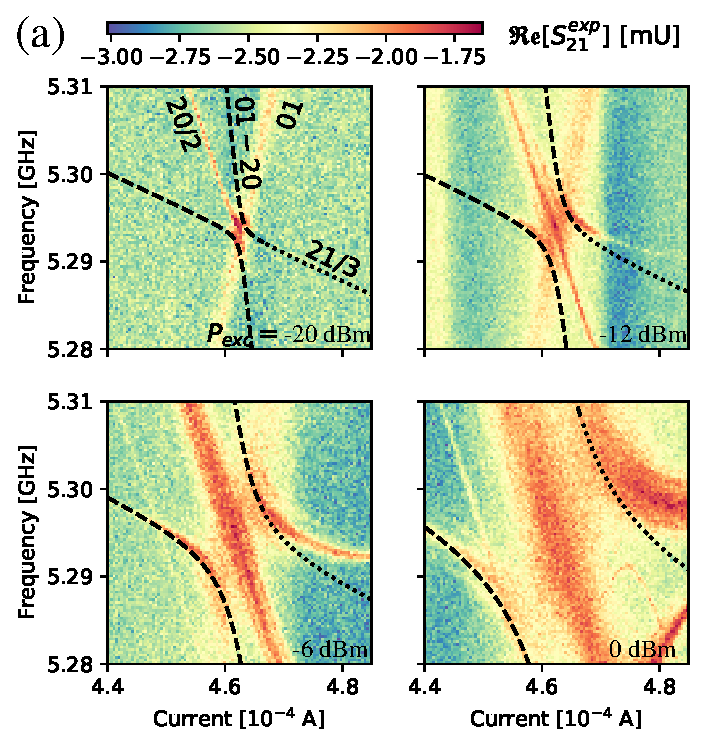
\includegraphics[width=.49\linewidth]{powerscan}
	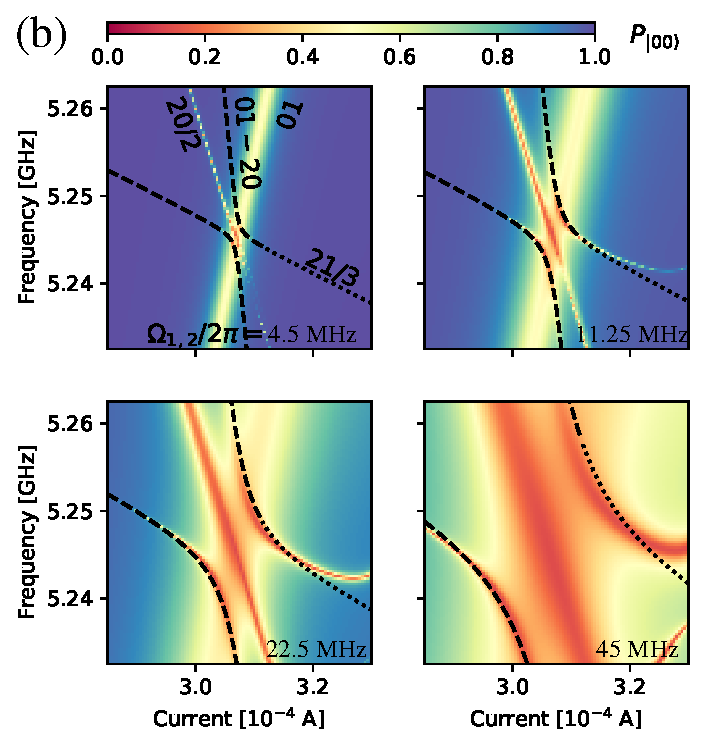
\includegraphics[width=.49\linewidth]{zoom2_picture}
	\caption{Power dependence of feature II: experiment and theory. Dashed are the model curves turning to dotted when the model is not expected to be valid (see Sections \ref{sec:theory} and \ref{sec:münchhausen}); model values for $\Omega_2$ are the same for both (a) and (b): $\Omega_{2}/2\pi=$ 4.5, 11.25, 22.5 and 45 MHz. \textbf{(a)} Experiment (second cooldown; the parameters are different to those in \autoref{fig:experiment}). The power of the microwave source is increased from -20 to 0 dBm and the corresponding growth of the splitting and the widths of the spectral lines is observed. \textbf{(b)} Simulation with amplitudes of the driving $\Omega_{1,2}$ equal to the model values; other parameters as in \autoref{fig:two-tone}. Note that now colours show the population of the ground state.}
	\label{fig:zoom}
\end{figure*}

\begin{figure}
	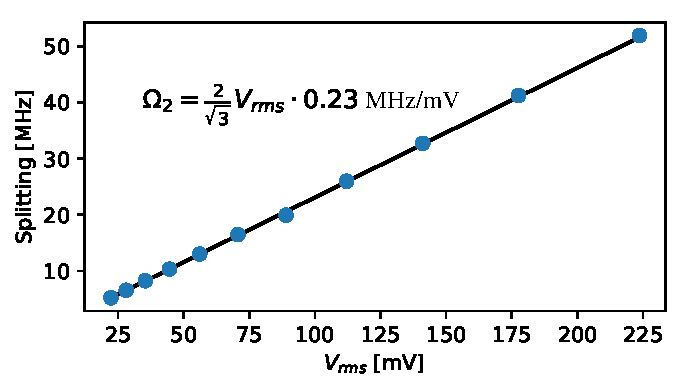
\includegraphics[width=\linewidth]{powerscan_1d}
	\caption{Linear dependence of the splitting size on the driving voltage of the microwave source $V_{rms} = \sqrt{10^{P_{exc}/10}\cdot 1 \text{ mW} \cdot 50\ \Omega}$, $\Omega_2 = V_{rms}\cdot 0.23$ MHz/mV. From Section \ref{sec:theory}, the splitting size is $\frac{2\sqrt{3}}{3} \Omega_2$.}
	\label{fig:splitting_linear}
\end{figure}

\begin{figure}
	\centering
	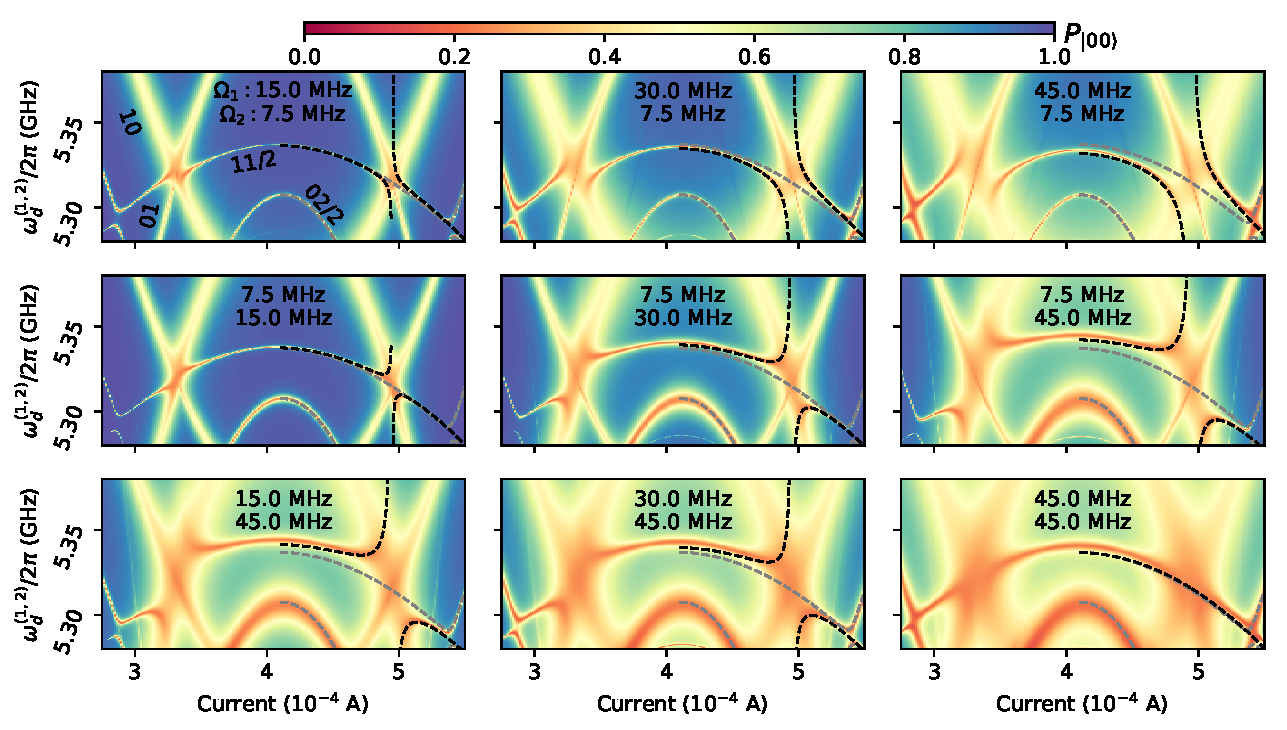
\includegraphics[width=\linewidth]{topological_splittings}
	\caption{Simulated population of the ground state when the transmons are driven at different amplitudes $\Omega_{1,2}$ but at the same frequency. In the left (right), $\Omega_{1(2)}$ is increased while $\Omega_{2(1)} = \text{const}$; two topologically different types of anticrossings arise depending on which transmon is driven stronger. Gray dashed lines show the stationary solution, in black are the model curves based on Sections \ref{sec:theory} and \ref{sec:münchhausen}.}
	\label{fig:difdrive}
\end{figure}


\subsection{Analysis of the spectra}

\paragraph{Identification of the spectral lines.} Though it is not possible to describe all of the experimental features with the stationary model, it is possible to use it to find which spectral lines correspond to which transitions in the system (see \autoref{fig:statinary_levels}). In \autoref{fig:two-tone}~(b), we have labelled the brightest lines with $ij/n$ where $i,j$ denote the final transmon states after the transition from the ground state, and $/n$ is optional for an $n$-photon process. We put the labels at the points where the SAM states are nearly factorized (dispersive regime for two coupled SAAs) and thus may be easily distinguished.

Due to the strong driving, we observe several multiphoton transitions besides the main lines at $\omega_{(1,2)}(\Phi_e)/2\pi$. The ${02/2}$ and ${20/2}$ are very common for transmons and lie $|\alpha_{(1,2)}|/2$ lower than the main lines $\omega_{(1,2)}(\Phi_e)$. Another two-photon process appears as $11/2$ line when two qubits are excited simultaneously. This process is used, for example, for doing the bSWAP gate\cite{poletto2012entanglement}; in our case, it is taking part in formation of feature I. A three-photon process $12/3$ is also clearly visible just below the $02/2$ line. As we will see, it is involved in forming features II and III. Notably, transitions $11/2$ and ${12/3}$ are forbidden when there is no interaction ($J=0$). Therefore, it is expected that all Roman-numbered features should only appear with non-vanishing $\hat H_{int}$.

When two lines intersect, they may form an avoided crossing if the corresponding matrix element of $\hat H_{int}$ is non-zero. In such cases, the SAM becomes inseparable with some of the eigenstates becoming superpositions of the factorized states. For a two-transmon SAM, such points are, for instance, crossings between ${01}$, ${10}$ or $ {11} $, $ {02} $($ {20} $). Additionally, marked as feature 3 in \autoref{fig:two-tone}, we see an avoided crossing between ${12}/3,\ {21}/3$ at the same $\Phi_e$ where ${01}$, ${10}$ intersect.


\paragraph{Features I, II and III.} First, we have focused on the feature III and have reproduced this avoided crossing in an additional numerical simulation taking only 2 levels for the transmon 1 and three levels for the transmon 2. Upon this, it has become clear that feature II and feature III actually are of the same nature and differ only by the ordering of the transmons: for II, they appear whence the transition ${01}$ intersects with the two-photon one ${20/2}$ (${10}$ intersects ${02/2}$ in III); one can see this clearly in \autoref{fig:two-tone}~(b).

From \autoref{fig:statinary_levels} we conclude that avoided crossing in III is between two transitions: ${12/3}$ and ${10} - {02}$ which are of the same frequency when $\omega_1 = \omega_2+\alpha_2/2$. The latter process is discernible in \autoref{fig:statinary_levels} as it depopulates ${10}$, but is not visible in \autoref{fig:two-tone}. In II, the reversed is true: ${21/3}$ and ${01} - {20}$ are crossing when $\omega_2 = \omega_1+\alpha_1/2$. From additional measurements and simulations, we have found that the size of these anticrossings depends on the driving power; the experimental and simulated results for II are shown in \autoref{fig:zoom}~(a), (b). As one can see, the growth of the splitting with increasing power is linear: its width is roughly equal to the FWHM of the ${01}$ spectral line which is approximately $\Omega_2/2\pi$ Hz. To fully quantify the shape of this splitting, in Section \ref{sec:theory} we derive analytical expressions for the dashed curves fitting the spectral lines in \autoref{fig:zoom}. By measuring the dependence of the splitting size on the microwave power we confirm its proportionality to the signal amplitude (see \autoref{fig:splitting_linear}).

We see a similar behaviour for feature I: increasing drive amplitude on one of the transmons while keeping the other one small and constant again elicits avoided crossings with the proportional size. In \autoref{fig:difdrive} we show only the simulation results; an experiment is not possible with our sample because there is no way to adjust the driving amplitudes $\Omega_{1,2}$ individually. We note that two qualitatively different patterns arise depending on which of the transmons is driven stronger than the other. From this and from the shape of the splitting in feature I of \autoref{fig:experiment}~(a), we can infer that $\Omega_1 \approx 2\Omega_2$ there.

These observations mean that I -- III are caused by light dressing. In the case III, the first transmon is dressed by a strong resonant field; in case II, the second one; finally, in case I, both transmons are dressed at the same time. We will discuss these effects in greater detail in \autoref{sec:theory}.

\paragraph{Secondary features.} Using \autoref{fig:statinary_levels}, we can get an insight into the features 1 -- 5 as well. 

Feature 1 is a small avoided crossing between ${02/2}$ and ${21/3}$. It is missing in the stationary solution and thus is caused by the light dressing just as I -- III. Feature 2 is its twin: ${12/3}$ and ${20/2}$ intersect there but the anticrossing is smaller due to the asymmetry of the driving strengths and is not resolved. 

Feature 3 is a large avoided crossing between three-photon processes ${12/3}$ and ${21/3}$. It is predicted by the stationary model, and direct diagonalization yields the splitting of $\frac{4}{3}J$. A remarkable detail here is that the dim lower branch implies the presence of a dark state with respect to the driving operator in the third order. 

Feature 4 is also explained by the stationary model and is caused by several spectral lines and a pair of avoided crossings near a single point (dotted lines in \autoref{fig:statinary_levels}). It appears at the point where ${02/2}$ intersects ${20/2}$ and is just barely visible in the experimental data because of the noise. Feature 5 is located at the intersection between ${20/2}$ and normally invisible ${10} - {02}$, and can be found in the experimental data, too. 

Finally, when the coupling is turned off ($J=0$) in the simulation, the system does not demonstrate any of the described details. This means that all these effects can only be attributed to the SAM as a whole. 

\subsection{Explaining extra avoided crossings}\label{sec:theory}

Since we had already connected the additional avoided crossings with the light dressing, it was natural to expect the Autler-Townes effect to be at the root of the avoided crossings. For a three-level system, the standard A-T effect is reviewed in Appendix \ref{sec:3-level-at}. However, in our case the level structure and the effect itself are more complicated. 

First of all, since during the spectroscopy we apply only a single microwave tone ($\omega_d^1 = \omega_d^2$), for the A-T effect it has to be simultaneously the coupler and the probe; the latter must be much weaker than the former, as well. These conditions are satisfied when $\omega_{(2,1)} = \omega_{(1,2)}+\alpha_{(1,2)}/2$  where we can simultaneously excite transitions $01 (10)$ and $20/2 (02/2)$ (features II and III, respectively) because the of the two-photon probe. Since the two-photon Rabi frequency is much smaller than the single-photon $\Omega_2$, it is natural to view this two-photon excitation as the probing process which does not affect the level structure. In contrast, the single-photon excitation is enough to dress the system. In other words, in our case the A-T coupling operator is $\hat H_{d}^1$ (strong), and the probing operator is $\hat H_{d}^2$ (weak in the two-photon regime). Their separation in our case is not in frequency but in the Hilbert subspaces they act upon.

Similarly, for feature I, the simultaneously excited transitions are $01 (10)$ and the two-photon $11/2$. However, as we have demonstrated in \autoref{fig:difdrive}, for the avoided crossings in I to be clearly observed it is required that $\Omega_{(1,2)} \gg \Omega_{(2,1)}$. 

Below, we give the detailed explanation of features II and III, and finally, I.

\begin{figure}
	\centering
	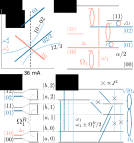
\includegraphics[width=\linewidth]{main_scheme_2}  
	\caption{Explaining feature III. \textbf{(a)} Schematic of the transition frequencies near III (not to scale). Red dashed line shows the current (0.36 mA) where the first transmon (orange) is below the second one (blue) exactly by $\alpha_2/2$ and several transitions become resonant. So far we assume that each transmon is driven at its own frequency. \textbf{(b)} System level structure at the resonant point including the driving $\hat H_{d}^1$ of the first transmon by a strong signal of amplitude $\Omega_1$ (orange ellipses) at a small detuning $\Delta_1$ from $\omega_1$. The second transmon driving is not shown here. Action of $\hat H_{int}$ in RWA is depicted as orange-blue circles. \textbf{(c)} In the frame rotating with the drive of the first transmon, all the states $\ket{0j},\ket{1j}$ become nearly degenerate ($\omega_1 \rightarrow \Delta_1$). Dressing by the strong excitation increases this splitting to $\Omega_1^R = \sqrt{\Omega_1^2 + \Delta_1^2}$. \textbf{(d)} Transitions in the light-dressed system when the second qubit is excited (level subspaces coupled by $\hat H_{d}^2$ are shown with blue ellipses). In the left part of the panel, all possible two-photon transitions near $\omega_1$ are depicted: the green transitions are not shifted in frequency, the red are red-shifted by $\Omega^R_1/2$ and the blue are blue-shifted by $\Omega^R_1/2$. In the right part, the most contributing trajectories are depicted; red crosses show transitions that are forbidden without the coupling $J$.}
	\label{fig:main_scheme}
\end{figure}

\begin{figure}
	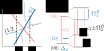
\includegraphics[width=.9\linewidth]{topo_scheme}
	\caption{Explaining feature I. (a) Schematic of the transitions near I. (b) Transitions in the frame rotating with the second transmon with dressing. As will be shown in Section \ref{sec:münchhausen}, in our experiment there can only be one visible transition to the left or to the right from the resonance.}
	\label{fig:featureI}
\end{figure} 

\paragraph{Features II and III.}  

In \autoref{fig:main_scheme}, we elaborate on how exactly the A-T effect occurs for feature III. For simplicity, we will temporarily assume that each transmon is driven at its own frequency (this assumption will be lifted in the following section). For convenience, in \autoref{fig:main_scheme}~(a) we schematically reproduce the transitions near III where the first transmon (orange) is below the second (blue), and the resonance point in current is shown with dashed red line. Next, \autoref{fig:main_scheme}~(b) demonstrates the stationary level structure of the SAM at 0.36 mA. Nearly-resonant with $10$ (detuning $\Delta_1$) single-photon driving with $\hat H_d^1$ is shown with orange ellipses while much weaker two-photon $\hat H_d^2$ is not shown yet. Since from numerical simulations we know that the third level of the first transmon is not necessary to observe the splitting, $\ket{02}$ is shown transparent, and hereinafter the states $\ket{j2},\ j=0..2$ are not used in the modelling.

The next step is to view the system in the frame rotating with the first transmon (\autoref{fig:main_scheme}~(c)) and then move to the  dressed picture similarly to Appendix \ref{sec:3-level-at}. Now, the first transmon splitting equals $\Omega_{1}^R = \sqrt{\Omega_1^2+\Delta_1^2}$, and its the new eigenstates (dressed states) are denoted $\ket{a}$ and $\ket{b}$. Meanwhile, the second transmon energies stay the same.


Finally, in \autoref{fig:main_scheme}~(d) we demonstrate possible two-photon transitions between the resulting eigenstates due to $\hat H_{d}^2$. In the left part of the panel, the unmodified transition at $\omega_1$ and two sidebands at $\omega_1 \pm \Omega_1^R/2$. The right part describes the mechanism of these two-photon processes through virtual excitations of the intermediate states. From here it becomes obvious that without the transmon-transmon interaction the sideband transitions are forbidden due the selection rule: $\bra{a,j}\hat{\mathbbm{1}}\otimes \hat n_2 \ket{b, j+1} = 0$ since $\braket{a}{b} = 0$. However, we will show that they become allowed in the second order in $J$ when the coupling is turned on.  Remarkably, due to the two-photon nature of the transitions, the Autler-Townes splitting in this case will be just $\Omega_1^R$.

Now, we will repeat this reasoning using a quantitative mathematical model. We start from the initial Hamiltonian \eqref{Hsystem}. To move to the rotating frame with \eqref{eq:rotation} and apply the RWA, will use the following operator:
\begin{equation}
R = \exp[-i\omega_d^1 t (b^{\dagger}b+c^{\dagger}c)]
\end{equation}  
Note that we rotate both transmon subspaces simultaneously in contrast to what is shown in \autoref{fig:main_scheme} because below it will be convenient to have time-independent $\hat H_{int}$:
\begin{equation}
\begin{aligned}
\omega_{(1,2)} &\rightarrow \Delta_{(1,2)} = \omega_{(1,2)} - \omega_d^{1},\\
\hat H_{int} &\rightarrow J \left[\hat \sigma_+ \hat c + \hat \sigma_-\hat c^\dag \right],\\
\hat H_{d}^1 &\rightarrow \frac{\Omega_1}{2} \hat \sigma_x,\ 
\hat H_{d}^2 \rightarrow \frac{\Omega_2}{2}(\hat c e^{i\delta t}  + \hat c^\dag e^{-i\delta t}),
\end{aligned}
\end{equation}
where $\delta = \omega_{d}^2 - \omega_{d}^1$.

Since $\hat H_{d}^1$ is now time-independent, we can move to the dressed basis by applying a transformation $\hat S$ which diagonalizes the first transmon. After that, the Hamiltonian may be split into three parts:
\begin{equation}
\begin{aligned}
\hat H^{D} &= \left[\frac{\Delta_1}{2} \hat{\mathbbm{1}}+\frac{\Omega_1^R}{2}\hat \sigma_z\right] + \Delta_2 \hat b^{\dagger}\hat b +\frac{1}{2}\alpha_2 \hat b^{\dagger}\hat b(\hat b^{\dagger}\hat b-1),\\
\hat V_J &= \hat S^\dag \hat H_{int}\hat S,\\
\hat V_t &= \hat S^\dag \hat H_{d}^{2} \hat S \equiv \hat H_{d}^{2}.
\end{aligned}
\end{equation}
The first part is diagonal, and the remaining two will be treated as perturbations. To simplify futher calculations, we take the working point where $\Delta_1 = 0$ and $\Delta_2 = - \alpha_2/2$. In these conditions, $H^D$ becomes degenerate as can be seen below in \eqref{eq:ham_matrix}:


Using the degenerate perturbation theory with $\hat V_J$ summarized in Appendix \ref{sec:dpt}, we have found the first-order corrected wave functions of $\hat H^D$, labelled $\ket{k},\ k=1..6$. 

The theory for two-photon processes is given in Appendix \ref{sec:2pp}. The probability rate of two-photon transition per unit interaction time using corrected eigenstates $\ket{k}$ and neglecting small terms we obtain:

\begin{equation}
A^{(2)}_{1\rightarrow 6} =\pi\Omega_2^4 \frac{16 J^4 \left(3 \alpha_2 ^2+7 \text{$\Omega_1
		$}^2\right)^2}{\alpha_2 ^{10}}
\end{equation}
\begin{equation}
A^{(2)}_{2\rightarrow 5} =\pi\Omega_2^4 \frac{4 J^4 (5 \alpha_2 +3 \text{$\Omega_1$})^2}{\alpha_2 ^8}
\end{equation}
From here it follows that in the studied SAM the sideband transitions are prohibited without interaction $(J=0)$ even in the second order, and the avoided crossing we are interested can not be observed.

\paragraph{Feature I.} Finally, we discuss the last of the dressing effects observed in the SAM. Its explanation is illustrated in \autoref{fig:featureI} for the case when $\Omega_2 \gg \Omega_1$. In this case, the second qubit is dressed, and the splitting has the shape shown in \autoref{fig:featureI}~(a). For the opposite case, the explanation is the same. As one can see, only the two-photon transition $11/2$ is affected. When the transitions $01$ and $10$ are close resonance, its frequency is $\omega_{11/2} \approx \omega_1 \approx \omega_2$ Similarly to the previous case with II and III, in the dressed basis, this transitions becomes a single-photon doublet transition for $\hat H_d^2$ located at $\omega_1 \pm \Omega_2^R$, see \autoref{fig:featureI}~(b). Note that in the experiment with only a single excitation frequency, it is not possible to observe both transitions at the same magnetic flux, and this is clearly visible in \autoref{fig:difdrive}. Instead, we observe one line to the left and the other to the right from the $01-10$ intersection. This behaviour will be explained in the following section.




\subsection{Self-consistent equations for the avoided crossings}
\label{sec:münchhausen}

Before, we have assumed that the transmons are driven independently at two different frequencies. In this section, we will employ the same model from \autoref{fig:main_scheme} to explain the experimentally observed splittings when only a single frequency $\omega_d$ is sent at the SAM. 

\paragraph{Features II, III.}As shown in \autoref{fig:main_scheme}~(d), the sideband transitions are formed by two-photon processes for $\hat H_d^2$. On the other hand, we know from the stationary solution that in the laboratory frame the two transitions forming the avoided crossing are $10 - 02$ (one-photon) and $12/3$ (three-photon). This means that there should be a smooth transformation between 1-, 2- and 3-photon processes when the system approaches the resonant point. Let's consider two-photon transitions $(10 - 02)/2$ and $12/2$. In the frame rotating with the first qubit (like in \autoref{fig:main_scheme}~(c)) when $\Omega_1$ = 0 (no driving yet on the first qubit), their frequencies are:
\begin{equation}
\begin{aligned}
\omega_{(10-02)/2} &= (\alpha_2 + 2 \omega_{2} - \Delta_1)/2,\\
 \omega_{12/2} &= (\alpha_2 + 2 \omega_{2} + \Delta_2)/2.
\end{aligned}
\end{equation}
When the first transmon becomes dressed by $\Omega_1 \neq 0$, its splitting $\Delta_1$ changes to $\Omega^R_1 =\sqrt{\Omega_{1}^2 + \left(\omega_{1} - \omega_{d}\right)^{2}}$. At this point it becomes clear that at the resonant point where $\alpha_2 + 2 \omega_{2} = 2\omega_1$, $\omega_{(10-02)/2}$ and $\omega_{12/2}$ are exactly equal to the two-photon sideband frequencies $\omega_1 \pm \Omega_1^R/2$ established above and thus should be used to model the splitting behaviour.

Since we are simultaneously dressing the states by $\hat H_d^1$ and probing two-photon transitions between them with $\hat H_d^2$ both at $\omega_d$, self-consistent equations have to be solved to find at which $\omega_d$ the sideband spectral lines will appear:
\begin{equation}
\begin{aligned}
\omega_{(10-02)/2} &= \omega_d,\\
\omega_{12/2} &= \omega_d
\end{aligned}
\end{equation}

When $\Omega_1 = 0$, these equations yield indentical pairs of solutions due to the properties of the modulus $|\omega_1 - \omega_d|$. Intriguingly, they are the three-photon and single-photon transition frequencies in the laboratory frame:
\begin{equation}
\omega_d = \begin{cases} \frac{\alpha_2}{3} + \frac{2 \omega_{2}}{3} + \frac{\omega_{1}}{3}, \\ \alpha_2 + 2 \omega_{2} - \omega_{1}\end{cases}
\end{equation}
When $\Omega_1 \neq 0$, we obtain the following solutions:
\begin{equation}
\omega_d = \frac{2 \alpha_2}{3} + \frac{4 \omega_{2}}{3} - \frac{\omega_{1}}{3} \pm \frac{\sqrt{3 \Omega_{1}^{2} + \left( \alpha_2 + 2 (\omega_{2} - \omega_{1})\right)^{2}}}{3}
\label{eq:splitting_model}
\end{equation}
The minimal splitting between these lines is found at the resonant point and equals $\frac{2 \sqrt{3}}{{3}} \Omega_1$. All these calculations may be repeated exactly for the feature II by reversing the order of the transmons; in that case, the maximal splitting will be $\frac{2 \sqrt{3}}{{3}} \Omega_2$

We find excellent agreement between our analytical model \eqref{eq:splitting_model} and both the experimental and simulated data as can be seen in \autoref{fig:zoom}. To plot the model curves we have fitted the $\omega_{(1,2)}(\Phi_e)$ transitions with simple linear functions and substituted them in \eqref{eq:splitting_model}; $\alpha_1$ is known from spectroscopy. The only free parameter left was $\Omega_2$. We have repeated this approximation for a range of microwave powers to confirm the linear dependence of the splitting on excitation amplitude (see \autoref{fig:splitting_linear}).

The upper branch is expected to deviate from the model (see dashed curves in \autoref{fig:zoom}) because of the avoided crossing marked as the secondary feature 3 which was not incorporated in the simple linear model. The small discrepancy between the experimental and simulated data in the upper branch is caused by a slight elevation of the lower sweet spot of the first transmon moving the avoided crossing 3 closer to the feature II; however, it is not important for our reasoning.	


\paragraph{Feature I.} Feature I may be explained using the same dressing model. Looking at \autoref{fig:featureI} for the case $\Omega_2 \gg \Omega_1$, we can write the other pair of self-consistent equations:
\begin{equation}
\omega_{1} \pm \Omega_2^R = \omega_d.
\end{equation}
Due to the fact that $\Omega_2^R = \sqrt{\Omega_2^2 + (\omega_2 - \omega_d)^2}$, these equations only have the same single solution:
\begin{equation}
\omega_d = \frac{\omega_1 + \omega_2}{2} - \frac{ \Omega_{2}^{2}}{2 \left(\omega_{1} - \omega_{2}\right)},
\label{eq:topo_1}
\end{equation}
which gives back the frequency of $11/2$ in the laboratory frame when $\Omega_2$ is zero. When $\Omega_2$ is non-zero, the solution near the point $\omega_1 \approx \omega_2$ is a hyperbolic curve, which agrees well with the numerical simulation. However, due to the finite coupling $J$ between the transmons, they never reach each other in frequency, and thus this model is not applicable when $|\omega_1 - \omega_2| \leq J$.

When $\Omega_1 \gg \Omega_2$, besides the replacement $\Omega_2 \rightarrow \Omega_1$, the equation \eqref{eq:topo_1} changes the sign:
\begin{equation}
\omega_d = \frac{\omega_1 + \omega_2}{2} + \frac{ \Omega_{1}^{2}}{2 \left(\omega_{1} - \omega_{2}\right)},
\label{eq:topo_1_inv}
\end{equation}
yielding the reversed shape of the splitting.

Continuing this logic, we can write down the resonance condition in the doubly-rotating frame when both transmons are dressed simultaneously:
\begin{equation}
\Omega_1^R \pm \Omega_2^R = 0.
\end{equation}
Solving it for $\omega_d$, we obtain the generalization of \eqref{eq:topo_1} and \eqref{eq:topo_1_inv}:
\begin{equation}
\omega_d = \frac{\omega_{1} - \omega_{2}}{2} + \frac{\Omega_{1}^{2} - \Omega_{2}^{2}}{ 2\left(\omega_{1} - \omega_{2}\right)}
\label{eq:topo_comm}
\end{equation}

The equation \eqref{eq:topo_comm} is used to plot the black dashed curves in \autoref{fig:difdrive} taking the $\Omega_{1,2}$ values from the simulation parameters shown therein. The frequencies $\omega_{1,2}$ are extracted from the fits to the visible spectral lines. We find good agreement between the model and the simulated data.

\appendix

\section{Standard Autler-Townes effect for a three-level atom} \label{sec:3-level-at}

The underlying cause of the A-T effect is the dressing of the atomic levels by strong EM radiation. There are two equivalent mathematical models for it: the light may be classical or quantized.

\begin{figure}
	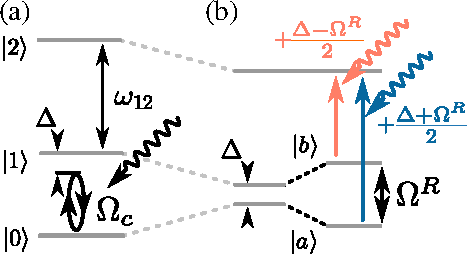
\includegraphics[width=\linewidth]{intro_scheme}
	\caption{Illustrating the A-T splitting by  the classical driving in the rotating frame ($\hbar=1$ here). \textbf{(a)} A three-level system is driven strongly by a ``coupler'' tone of amplitude $\Omega$ at frequency $\omega_{01}-\Delta$ which induces Rabi oscillations between $\ket{0}$ and $\ket{1}$ at the generalized Rabi frequency $\Omega_R = \sqrt{\Omega^2 + \Delta^2}$. \textbf{(b)} Moving to the frame rotating with the drive, we effectively change the $\ket{0}\rightarrow \ket{1}$ transition frequency to $\Delta$. However, when the RWA is applied and Hamiltonian is re-diagonalized, the splitting between two lowest levels (dressed states $\ket{a}$ and $\ket{b}$) becomes $\Omega^R$. Now, the experimenter may observe a doublet transition from these levels to the state $\ket{2}$ at frequencies $\omega_{12}+(\Delta \pm \Omega^R)/2$.} 
	\label{fig:at-standard}
\end{figure}

\paragraph{Classical derivation.} In the classical case, the mathematical description goes as follows. At first, there is a three-level system which is driven by a strong radiation with an amplitude $\Omega_1$ at a frequency detuned by $\Delta$ from the $\ket{0}\rightarrow \ket{1}$ transition with a frequency $\omega_{01}$ (the \textit{coupler} tone). Additionally, we have a weak probe radiation at a frequency $\omega_{p}$ and with an amplitude $\Omega_2$ between $\ket{1}$ and $\ket{2}$ (the \textit{probe} tone). This step is illustrated in \autoref{fig:at-standard}~(a). The Hamiltonian for such system is as follows:

\begin{equation*}
\hat H^c_0 = \left[\begin{matrix}
0 & \Omega_{1} \cos{\left(\omega_{01}- \Delta \right)t} & 0\\
\Omega_{1} \cos{\left(\omega_{01} - \Delta \right)t}   & \omega_{01} &\Omega_{2} \cos\omega_p t  \\
0 & \Omega_{2} \cos{\omega_p t}  & \omega_{02}\end{matrix}\right].
\end{equation*}

Next, we move to the rotating frame by using an operator
\[
\hat R = \left[\begin{matrix} 
1 & 0 & 0\\0 & e^{i t \left(\omega_{01}- \Delta\right)} & 0\\0 & 0 & e^{i t \left(\omega_{01}- \Delta\right)}\end{matrix}\right].
\]
Note here that level $\ket{2}$ is also rotated: this is convenient to preserve the frequency of the driving term with $\Omega_2$. The new Hamiltonian should be calculated as follows: $\hat H_1 = \hat R^\dag \hat H_0 \hat R + i \dot{\hat{R}}^\dag \hat R$. The level structure without driving  is shown in the left part of \autoref{fig:at-standard}~(b). Applying the RWA, we obtain:
\begin{equation*}
\hat H^c_1 = \left[\begin{matrix}0 &\Omega_{1}/2 & 0\\\Omega_{1}/2 & \Delta & \Omega_{2} e^{i t \omega_p}/2\\0 & \Omega_{2} e^{-i t \omega_p}/2 & \omega_{02} - \omega_{01}+\Delta \end{matrix}\right].
\end{equation*}

Next, moving to the basis where the upper left 2x2 corner is diagonal (the right part of \autoref{fig:at-standard}~(b)), we obtain:

\begin{equation*}
\hat H^c_3 = \left[\begin{matrix} 
\frac{\Delta}{2} - \frac{\sqrt{\Delta^{2} + \Omega_{1}^{2}}}{2} & 
0 &
\frac{\Omega_{2} e^{i t \omega_{p}}}{2}\sin(\theta)
\\
0 & 
\frac{\Delta}{2} + \frac{\sqrt{\Delta^{2} + \Omega_{1}^{2}}}{2} & 
\frac{\Omega_{2} e^ {i t \omega_p}}{2}\cos(\theta)
\\
\frac{\Omega_{2} e^{-i t \omega_{p}} }{2}\sin(\theta) & 
\frac{\Omega_{2} e^{-i t \omega_{p}}}{2} \cos(\theta) & 
\omega_{12} +\Delta 
\end{matrix}\right].
\end{equation*}

One may see that now resonant conditions for the probe drive are $\omega_p = \omega_{12} + \dfrac{(\Delta \pm \Omega^R)}{2}$, where $\Omega^R = \sqrt{\Omega_1^2 + \Delta^2}$, $\omega_{12} = \omega_{02}- \omega_{01}$, and its amplitude is renormalized by an angle $\theta,\ \tan 2\theta = -\frac{\Omega_1}{\Delta}$.


\paragraph{Quantum derivation.} For the fully quantum interpretation, we model the incident radiation at the frequency $\omega_{01}-\Delta$ as a single-mode quantum oscillator which is coupled to the system. The Hamiltonian for this model will be as follows:
\[
\begin{split}
\hat H^q_0 = \omega_{01} \ket{1}\bra{1} + \omega_{02} \ket{2}\bra{2} + (\omega_{01}-\Delta) \hat a^\dag \hat a + \\\ g (\hat a^\dag + \hat a)\otimes (\ket{1}\bra{0}+\ket{0}\bra{1}),
\end{split}
\]
where $g$ is the coupling strength and $a$ is the photon annihilation operator. After moving to the rotating frame with $\hat R = \exp[i t (\omega_{01}-\Delta)(\hat a^\dag \hat a + \ket{1}\bra{1}+\ket{2}\bra{2})]$ and applying the RWA, the Hamiltonian transforms into
\[
\begin{split}
\hat H^q_1 = \Delta \ket{1}\bra{1} + (\omega_{12}+\Delta) \ket{2}\bra{2} + \\\ g \left[\hat a^\dag \otimes \ket{0}\bra{1} + \hat a \otimes \ket{1}\bra{0}\right].
\end{split}
\]
If we presume that the resonator is in a coherent state $\ket{\alpha e^{-it(\omega_{01}-\Delta)}}$ with $\langle N\rangle = \alpha^2$ photons and average $\hat H_1^q$ over the resonator subspace, we from the interaction term will obtain again the classical driving strength $\Omega_1 = 2 \sqrt{\langle N \rangle} g$ in correspondence with the classical driving case. Similarly, the energy levels $\ket{1, N-1}$ and $\ket{0, N}$ become mixed due to the coupling, and their splitting changes from $\Delta$ to $\Omega_R = \sqrt{\Omega_1+\Delta}$. The following steps completely reproduce the classical case if we add the probe tone $\Omega_2$ in the last equation.

\section{The dressed Hamiltonian in the matrix form}

\vspace{1cm}

\renewcommand{\kbldelim}{[}% Left delimiter
\renewcommand{\kbrdelim}{]}% Right delimiter
\begin{widetext}
	\begin{equation}
	\hat H^D + \hat V_J + \hat V_t  = \kbordermatrix{
		&\ket{a,0} & \ket{b,0} & \ket{a,1} & \ket{b,1} & \ket{a,2} & \ket{b,2} \\
		\ket{a,0}& -\frac{\Omega_1}{2} & 0 & \frac{\Omega_{2}e^{i \text{$\delta$} t}}{2} -\frac{J}{2} & \frac{J}{2} & 0 & 0 \\
		\ket{b,0} & 0 & \frac{\Omega_1}{2} & -\frac{J}{2} & \frac{\Omega_2 e^{i \delta t}}{2} + \frac{J}{2} & 0 & 0 \\
		\ket{a,1} &\frac{\Omega_2 e^{-i \text{$\delta$} t} }{2}  - \frac{J}{2} & -\frac{J}{2} & - \frac{\alpha}{2} - \frac{\Omega_1}{2}&
		0 & \frac{\text{$\Omega_2$} e^{i \text{$\delta$} t}}{\sqrt{2}} -\frac{J}{\sqrt2} & \frac{J}{\sqrt2} \\
		\ket{b,1} & \frac{J}{2} & \frac{\text{$\Omega_2$} e^{-i \text{$\delta $} t}}{2} +\frac{J}{2} & 0 & - \frac{\alpha}{2} + \frac{\Omega_1}{2} & -\frac{J}{\sqrt 2} & \frac{\text{$\Omega_2$} e^{i \text{$\delta
					$} t}}{\sqrt 2} + \frac{J}{\sqrt 2} \\
		\ket{a,2} & 0 & 0 & \frac{\Omega_2 e^{-i \delta t}}{2} - \frac{J}{\sqrt 2} & -\frac{J}{\sqrt 2} &
		-\frac{\Omega_{1}}{2} & 0 \\
		\ket{b,2} & 0 & 0 & \frac{J}{\sqrt 2} & \frac{\text{$\Omega_2$} e^{-i \text{$\delta $} t}}{\sqrt 2} + \frac{J}{\sqrt 2} & 0 & \frac{\Omega_{1}}{2}\\
	}
	\label{eq:ham_matrix}
	\end{equation}
\end{widetext}

\section{Degenerate perturbation theory} \label{sec:dpt}
\begin{equation}
H^R=H_0+V_J
\end{equation}
At our working point the equation $\Delta_2=\alpha/2$ is true and $H_0$ becomes degenerate. Let's consider our system in the basis of dressed states.
\begin{equation}
H_0^{d}= diag(-\frac{\Omega_{1}}{2},\frac{\Omega_{1}}{2},\frac{(-\alpha-\Omega_{1})}{2},\frac{-\alpha+\Omega_{1}}{2},-\frac{\Omega_{1}}{2},\frac{\Omega_{1}}{2})
\end{equation}
The choice of wave functions from a degenerate subspace is arbitrary because any linear combination of functions from this subspace will satisfy the Schrodinger equation. However, if we demand that the change of wave functions be small under the applied small perturbation, then the choice of wave functions become defined. To obtain correct wave functions we need to diagonalize $V_J^{d}$ in the degenerate subspace. However, we can notice that $V_J^{d}$ is identically the zero matrix in our subspace, so technically any choice of basis will diagonalize $V_J^{d}$. This means that the degeneracy is not lifted at first-order in perturbation theory. We have to pick eigenvectors which diagonalize following matrix:
\begin{equation}
	\begin{matrix}
	M_{nn'} = \sum_{m}\frac{V_{nm}V_{mn'}}{E_n-E_m}
	\end{matrix}
\end{equation}
Where $\ket{n}$ and $\ket{n'}$ are states with same energy $E_n$.  The sum is over all states $m$ not in the degenerate subspace.
For example, in our case for one of degenerate subspaces:
\begin{equation}
	M_{15} =\left[\begin{matrix}\frac{J^{2} \left(\Omega_{1} - \alpha\right)}{\alpha \left(2 \Omega_{1} - \alpha\right)} & \frac{\sqrt{2} J^{2} \Omega_{1}}{\alpha \left(2 \Omega_{1} - \alpha\right)}\\\frac{\sqrt{2} J^{2} \Omega_{1}}{\alpha \left(2 \Omega_{1} - \alpha\right)} & \frac{2 J^{2} \left(\Omega_{1} - \alpha\right)}{\alpha \left(2 \Omega_{1} - \alpha\right)}\end{matrix}\right]
\end{equation}
The normalized eigenvectors $(C_n,C_{n'})$ of the matrix will give the desired zero approximation wave-functions.
The first-order correction to the states from degenerate subspace:
\begin{equation}
	\ket{n^0}+\ket{n^1} = \sum_n C_{n}\ket{n^0} + \sum_{m\ne n}\ket{m^0}\frac{\bra{m^0}V\ket{n^0}}{E_n^0-E_m^0}
\end{equation}
The sum is over all states $n$ in the degenerate subspace $n=(n,n')$.
The first-order corrections for not degenerate state compute by using the ordinary perturbation theory.
\begin{equation}
	\ket{j^1} = \sum_{m\ne j}\ket{m^0}\frac{\bra{m^0}V\ket{j^0}}{E_j^0-E_m^0}
\end{equation}





\section{Theoretical description of two-photon process}\label{sec:2pp}
Perturbation theory allows semianalytical calculation of the transition rates for single and multi-photon processes\cite{faisal2013theory}.

Let's consider the Hamiltonian $H = H_0+V(t)$, with time-dependent interaction $V(t)$ and "reference" part -- $H_0$ and wave function $\Psi(t)$. After switching to the interaction picture $V(t)$ modifies to $\tilde{V}(t) = \exp(i H_0 t)V(t)\exp(-i H_0 t)$ and Schrödinger equation gives by $i \derivative{\psi(t)}{t}=\tilde{V}(t)\psi(t)$, where $\psi(t)=\exp(i H_0 t)\Psi(t)$. The reference states of $H_0$ will be denoted $\ket{j}$, $H_0 \ket{j} = \omega_j \ket{j}$ whence it follows that matrix elements  of the modified interaction take the form $\bra{j}\tilde{V}(t)\ket{i}=\exp(i(\omega_j-\omega_i)t)\bra{j}V(t)\ket{i}$. A "solution" of Schrödinger equation in interaction picture corresponding to the initial reference state $\ket{i}$ is

\begin{equation}\label{forpsi}
	\tilde{\psi_i}(t)=\ket{i} - i \int_{-\infty}^{t}dt_1\tilde{V}(t_1)\ket{\tilde{\psi_i}(t_1)}
\end{equation} 

Mainly important for us is to find not the wave function but the probability of transition from the initial state $\ket{i}\rightarrow\ket{f}$, where $\ket{f}$ is the final state. Firstly, we find the transition amplitude $A_{fi} = \bra{f}U(t,t_0)\ket{i}=\bra{f}\psi_i(t)$ where $U(t,t_0)$ evolution operator. 

Solving \autoref{forpsi} by simple iteration gives the series solution
\begin{equation}
	U(t,t_0) = 1+\sum_{n}U^{(n)}(t,t_0)
\end{equation}
\begin{equation}
	U^{(n)}(t,t_0) = -i^n \int_{t_0}^{t}d t_1\tilde{V}(t_1)...\int_{t_0}^{t_{n-1}}d t_n\tilde{V}(t_n)
\end{equation}
For "weak" interaction the series may be truncated to a fine term $n$ and the $n$th- order transition amplitude $\bra{f}U^{(n)}(t,t_0)\ket{i}$ can be evaluated. 
In our case the interaction in interaction picture satisfies the following relation
\begin{equation}
	\begin{split}
	\tilde{V}(t)=\exp(i H_0 t) \Omega\cos(\omega_d t)(\hat b+\hat b^{\dagger})\exp(-i H_0 t)\overset{RWA}{=}\\ \exp(i H_0 t) \Omega(\hat b^{\dagger} e^{-i\omega_d t}+\hat be^{i\omega_d t})\exp(-i H_0 t)
	\end{split}
\end{equation}
Taking the matrix element between the initial and the final states $\ket{i}$ and $\ket{f}$, one immediately obtains
\begin{equation}
	\begin{split}
	\bra{f}U^{(1)}(t,t_0)\ket{i}=-i\int_{t_0}^{t}dt_1\tilde{V}(t_1)=\\-i\frac{\Omega}{2}\big[\int_{t_0}^{t}dt_1e^{i(\omega_f-\omega_i-\omega_d)t_1}\bra{f}b^{\dagger}\ket{i}+\\
	\int_{t_0}^{t}dt_1e^{i(\omega_f-\omega_i+\omega_d)t_1}\bra{f}b\ket{i}\big]
	\end{split}
\end{equation}
To calculate second-order term we used the following expression $\sum_{j}\ket{j}\bra{j}=\mathbbm{1}$.
\begin{equation}
	\begin{split}
	\bra{f}U^{(2)}(t,t_0)\ket{i}=-\bra{f}\int_{t_0}^{t}dt_1\tilde{V}(t_1)\mathbbm{1}\int_{t_0}^{t_1}dt_2\tilde{V}(t_2)\ket{i}=\\-\int_{t_0}^{t}dt_1 e^{i(\omega_f-\omega_j)t_1}\bra{f}V(t_1)\ket{j}\int_{t_0}^{t_1}dt_2e^{i(\omega_j-\omega_i)t_2}\bra{j}V(t_2)\ket{i}
	\end{split}
\end{equation}
Go over the long-time limit $t\rightarrow\infty$ in the final integral and collect the terms belongings to the same delta functions. This gives
\begin{equation}
	\begin{split}
	\bra{f}U^{(2)}(\infty)\ket{i}=\\\frac{\pi i\Omega^2}{2}\bigg[\delta(\omega_f-\omega_i+2\omega_d)\sum_j\frac{\bra{f}b\ket{j}\bra{j}b\ket{i}}{\omega_j-\omega_i+\omega_d}+\\
	\delta(\omega_f-\omega_i)\bigg(\sum_j\frac{\bra{f}b^{\dagger}\ket{j}\bra{j}b\ket{i}}{\omega_j-\omega_i+\omega_d}+\\
	\sum_j\frac{\bra{f}b\ket{j}\bra{j}b^{\dagger}\ket{i}}{\omega_j-\omega_i-\omega_d}\bigg)+\\
	\delta(\omega_f-\omega_i-2\omega_d)\sum_j\frac{\bra{f}b^{\dagger}\ket{j}\bra{j}b^{\dagger}\ket{i}}{\omega_j-\omega_i-\omega_d}\bigg]
	\end{split}
\end{equation}
The probability of two-photon transition from state $\ket{i}$ to state $\ket{f}$ is simply the square modulus of the corresponding amplitude. So, $P^{(2)}_{i\rightarrow f}= |	\bra{f}U^{(2)}(\infty)\ket{i}|^2$.
The rate (probability per unit interaction time T) of absorption of $2$ photons is defined as:
\begin{equation}
	W^{(2)}_{i\rightarrow f}=\lim\limits_{T\rightarrow\infty}\frac{P^{(2)}_{i\rightarrow f}}{T}
\end{equation}
For simplifier the equation we have made use of the relation:
\begin{equation}\nonumber
	\delta(\omega_f-\omega_i-2\omega_d) =\frac{1}{2\pi} \lim\limits_{T\rightarrow\infty}\int_{-T/2}^{T/2}e^{i(\omega_f-\omega_i-2\omega_d)t}dt = \lim\limits_{T\rightarrow\infty}\frac{T}{2\pi}
\end{equation} 
For $\omega_f=\omega_i+2\omega_d$.
\begin{equation}\label{prob}
\begin{split}
	W^{(2)}_{i\rightarrow f}=\frac{\pi\Omega^4}{8}\bigg|\sum_j\frac{\bra{f}b^{\dagger}\ket{j}\bra{j}b^{\dagger}\ket{i}}{\omega_j-\omega_i-\omega_d}\bigg|^2\delta(\omega_f-\omega_i-2\omega_d)=\\ A^{(2)}_{i\rightarrow f}\delta(\omega_f-\omega_i-2\omega_d)
\end{split}
\end{equation}

\section{Measurement setup and methods}\label{sec:meas_setup}
The sample was measured in a BlueFors LD250 dilution refrigerator at 16 mK. For the readout a Keysight PNA-L N5232A VNA was used. For the coherent excitation of the SAM, we used an Agilent MXG N5183B analog signal generator. The sample was 
flux biased using Yokogawa GS200 current sources (two for the flux lines and one for the external coil wrapped around the sample).

Input microwave lines were isolated from high-temperature noise with 60 dB of attenuation (10 @ 4K, 10 @ 1K, 20 @ 100 and 16 mK) and custom-made IR filters. The additional on-chip attenuation (due to the small capacitive coupling) between the qubit drive line and the qubits was calculated in Sonnet to be around 70 dB @ 6 GHz. Coaxial flux-bias lines were attenuated by 20 dB @ 4K and IR filtered as well. Output path contained two 20 dB isolators and two amplifiers: the 4-14 GHz LNF amplifier at the 4 K stage and the room-temperature LNF amplifier.

As the main experimental method, we have employed the two-tone spectroscopy which consists of exciting the SAM with monochromatic light at certain frequency until steady state is reached while simultaneously measuring the signal transmission at the readout resonator frequency. This measurement yields the average value of the joint measurement operator $\hat M$ in the steady-state.

\section{Text}

In order to determine which transitions correspond to the lines, the stationary Schrödinger equation was solved \autoref{fig:spectr} in three-level approximation for both of qubits. With the Hamiltonian of the system:
\begin{equation}
	H_{system} = H_{tr1}\otimes \mathbbm{1}+\mathbbm{1}\otimes H_{tr2}+H_{int}
\end{equation}



\bibliography{papers_bibliography}% Produces the bibliography via BibTeX.	
\end{document}